\documentclass{article}

%% Page Margins %%
\usepackage{geometry}
\geometry{
    top = 0.75in,
    bottom = 0.75in,
    right = 0.75in,
    left = 0.75in,
}

\usepackage{amsmath}
\usepackage{graphicx}
\usepackage{parskip}

\title{Lab 2: The Design Hierarchy}

% TODO: Enter your name
\author{Frederick Meneses}

\begin{document}
\maketitle

\section*{Part I}

\begin{enumerate}
\item If the truth table in Table 2.1 of the handout was given in full, how many rows would it have?

$$2^6 \text{ rows.}$$
% TODO

\item Export the schematic of the mux4to1 subcircuit as an image and include it in your report.
% TODO

\begin{figure}[ht!]
    \centering
    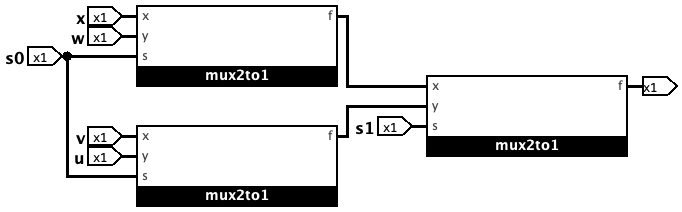
\includegraphics[width=0.7\textwidth]{part1.png}
    \caption{A schematic of the 4-to-1 multiplexer}
    \label{f:part1}
\end{figure}
\end{enumerate}

\section*{Part II}

\begin{enumerate}
\item Derive seven truth tables, one for each segment of the 7-segment decoder.
% TODO

\begin{table}[ht!]
\small
\centering
\begin{tabular}{c|c|ccccccc}
$D_{3:0}$& Character & $S_0$ & $S_1$ & $S_2$ & $S_3$ & $S_4$ & $S_5$ & $S_6$\\
\hline
0000 & 0 & 1 & 1 & 1 & 1 & 1 & 1 & 0\\
0001 & 1 & 0 & 1 & 1 & 0 & 0 & 0 & 0\\
0010 & 2 & 1 & 1 & 0 & 1 & 1 & 0 & 1\\
0011 & 3 & 1 & 1 & 1 & 1 & 0 & 0 & 1\\
0100 & 4 & 0 & 1 & 1 & 0 & 0 & 1 & 1\\
0101 & 5 & 1 & 0 & 1 & 1 & 0 & 1 & 1\\
0110 & 6 & 1 & 0 & 1 & 1 & 1 & 1 & 1\\
0111 & 7 & 1 & 1 & 1 & 0 & 0 & 0 & 0\\
1000 & 8 & 1 & 1 & 1 & 1 & 1 & 1 & 1\\
1001 & 9 & 1 & 1 & 1 & 1 & 0 & 1 & 1\\
1010 & A & 1 & 1 & 1 & 0 & 1 & 1 & 1\\
1011 & b & 0 & 0 & 1 & 1 & 1 & 1 & 1\\
1100 & c & 0 & 0 & 0 & 1 & 1 & 0 & 1\\
1101 & d & 0 & 1 & 1 & 1 & 1 & 0 & 1\\
1110 & E & 1 & 0 & 0 & 1 & 1 & 1 & 1\\
1111 & F & 1 & 0 & 0 & 0 & 1 & 1 & 1\\
\end{tabular}
\end{table}

\item Use Karnaugh maps to write seven Boolean functions for each segment so that they are optimized.
% TODO

\begin{align*}
    S_0 &= \overline{v}   \overline{x} + \overline{u}   w+ \overline{u}  v x+v w+u \overline{v}   \overline{w} \\
    S_1 &= \overline{u}  \overline{v} + \overline{u}   \overline{w}  \overline{x} + \overline{v}    \overline{x} + \overline{u}  w  x+u  \overline{w} x\\
    S_2 &= \overline{u}  \overline{w} + \overline{u}  x+ \overline{w} x+ \overline{u}   v+u  \overline{v} \\
    S_3 &=  \overline{u}  \overline{v}  \overline{x} + \overline{u} w   \overline{x} + \overline{v}  w  x+v \overline{w}   x+u  \overline{w} +uv  \overline{x} \\
    S_4 &=   \overline{v} \overline{x} +w \overline{x} +u  w+u v\\
    S_5 &=  \overline{u}  \overline{w}  \overline{x} + \overline{u}   v \overline{w} + \overline{u}   v  \overline{x} +u  \overline{v} +u w \\
    S_6 &=  \overline{v}  w+v  \overline{w} +v  \overline{x} +u \\
\end{align*}

\item Use the naming scheme \verb|HEX0|, \verb|HEX1|, ..., \verb|HEX6| for each subcircuit.
    Export each subcircuit schematic as an image and include it in your report.
% TODO

\begin{figure}[ht!]
    \centering
    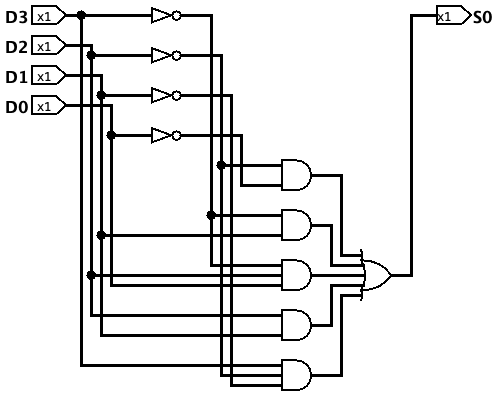
\includegraphics[width=0.7\textwidth]{part2_hex0.png}
    \caption{A schematic of HEX0}
    \label{f:part2_hex0}
\end{figure}

\begin{figure}[ht!]
    \centering
    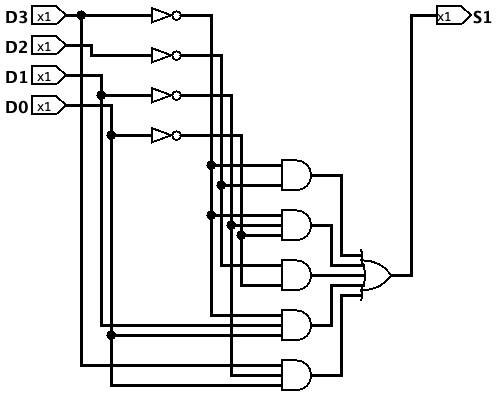
\includegraphics[width=0.7\textwidth]{part2_hex1.png}
    \caption{A schematic of HEX1}
    \label{f:part2_hex1}
\end{figure}

\begin{figure}[ht!]
    \centering
    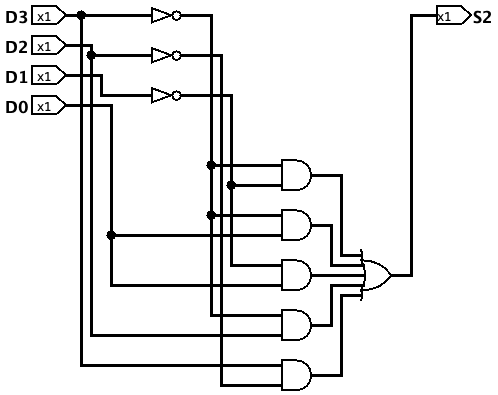
\includegraphics[width=0.7\textwidth]{part2_hex2.png}
    \caption{A schematic of HEX2}
    \label{f:part2_hex2}
\end{figure}


\begin{figure}[ht!]
    \centering
    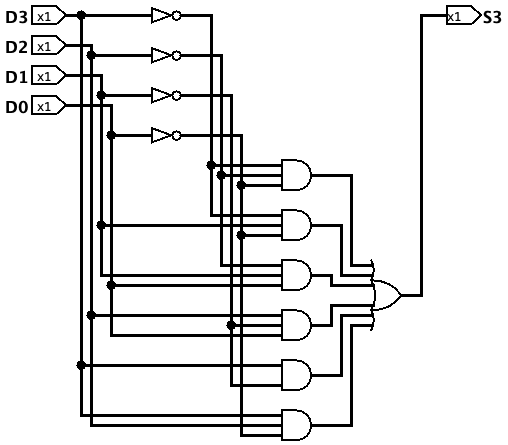
\includegraphics[width=0.7\textwidth]{part2_hex3.png}
    \caption{A schematic of HEX3}
    \label{f:part2_hex3}
\end{figure}

\begin{figure}[ht!]
    \centering
    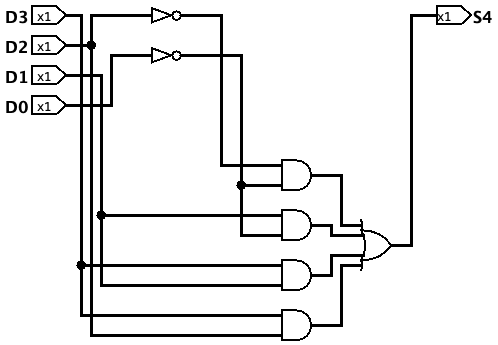
\includegraphics[width=0.7\textwidth]{part2_hex4.png}
    \caption{A schematic of HEX4}
    \label{f:part2_hex4}
\end{figure}

\begin{figure}[ht!]
    \centering
    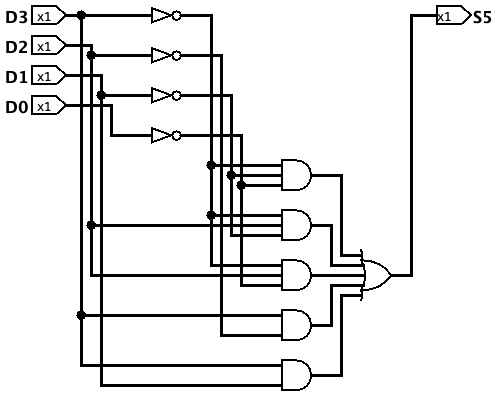
\includegraphics[width=0.7\textwidth]{part2_hex5.png}
    \caption{A schematic of HEX5}
    \label{f:part2_hex5}
\end{figure}

\begin{figure}[ht!]
    \centering
    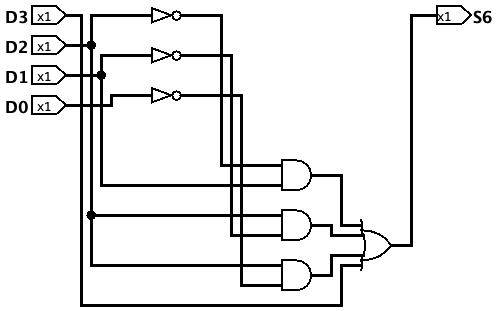
\includegraphics[width=0.7\textwidth]{part2_hex6.png}
    \caption{A schematic of HEX6}
    \label{f:part2_hex6}
\end{figure}

\end{enumerate}

\end{document}